\articlehead{Species Selection and Character Creation}{Makyo}{2013}

This weekend, I had the privilege of helping facilitate a panel at Rocky Mountain Fur Con 2013 surrounding the topic of species selection and character creation. The panel was a delightful discussion about the ways in which we build up the avatars we use to interact within our subculture, and why exactly it is that we choose the animal (or animals) that we become with our character (or characters).

That's not all, though. I also had the privilege of sitting down with Klisoura, [a][s] contributor of Furry Survey fame, and having not only several delightful discussions on topics as diverse as tennis balls and coyotes, but also a little impromptu hack-a-thon in the hotel lobby on the subject of species selection. This tied in well enough with the panel that some of the results of that were shown during the Q\&A after the discussion, and even led to several other conversations with various different furries over dinner and the next day. The whole weekend was a blast, but I'd like to tie up some of these conversation threads and ideas into something worth showing here on [a][s].

The title of that particular panel was the same as this post, ``Species Selection and Character Creation'', and was intended to be something new for me, and, I felt, relatively new for the convention as well. Rather than sit behind the table at the head of the discussion room and dictate a set of ideas to an audience, my goal was to re-arrange the chairs in the room into a circle and have everyone participate evenly in a sort of Socratic-style exploration of species and avatar. However, given the hour of sleep I'd had the night before, it worked out somewhere in between. While the Socratic ``asking questions to receive answers everyone already knows about themselves'' part worked out pretty well, I wasn't able to make real the truly participatory experience of everyone being able to see each other. I offer this as an explanation for not simply posting the audio from the panel itself, though it was recorded. If I get around to mastering the audio well enough to make it presentable, I'll post it here and make note of it. I think it's worth a listen!

I began by asking the room full of furries why they chose the animal they did for their species, and I received a lot of answers that fit in well with my experience of the fandom. Notable among the explanations were the oft-used words `identity', `connection', `personality', and `characteristics'. And this, of course makes sense. Many introductions to furry, whether they're websites (the first introductory website I found was Captain Packrat's explanation of FurCodes) or friends, explain that although furry is about being a fan of anthropomorphism in general, it often (but not always) specifically involves a personal connection with an animal that leads to the creation of a personal character: an avatar often used in interaction with other furries.

We all know this, of course, but it's always interesting to see the data bear it out. A discussion with Klisoura prior to the panel led to an experiment: is such a thing visible in the answers provided by respondents to the furry survey? It turns out that it is, in its own way. On the survey, users are asked the species of their character or characters, and then given room to provide an explanation of just why they chose the species they did. Free-text answers are hard to parse down into simple one-way conclusions, and are not necessarily available to be shared as they stand. However, we can draw conclusions about the use of language itself within these answers, and in this instance, we did so by means of one of the simpler means of textual analysis: frequency counts.

We've analyzed the responses for many of the most popular species represented in the responses to the 2012 Furry Survey. Breaking this down by species not only helps us spot keywords such as mentioned above, but also helps us see where additional words, especially emotionally or spiritually charged words, are used when identifying with particular species. Let's start out with one of the easier ones, for huskies, where I can point to a few of these words in particular to explain what I mean:

\begin{figure}
  \begin{center}
    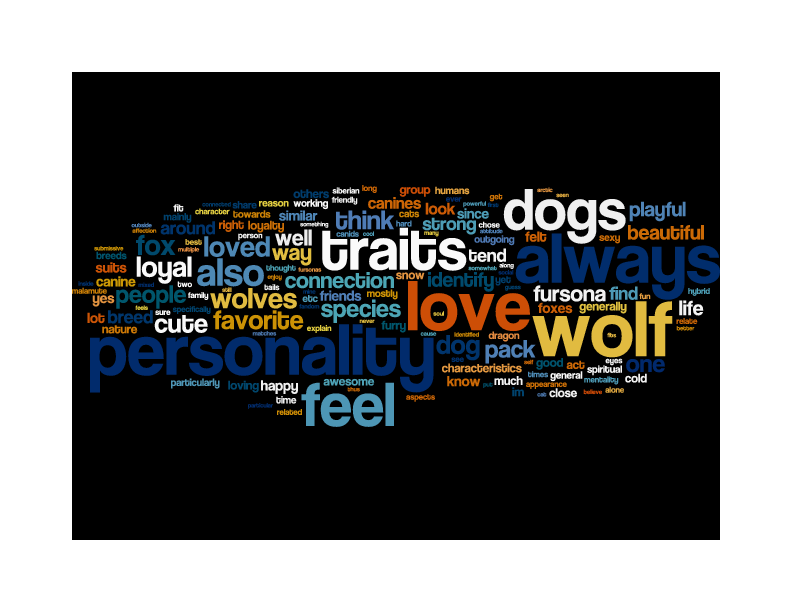
\includegraphics[width=\textwidth]{content/assets/species--husky}
  \end{center}
  \caption{Husky word-cloud}
\end{figure}

We see our previously tagged set of words such as `traits', `personality', and `always' (left in\footnote{The responses were cleaned of some very common words that tended to skew the word-clouds, such as articles (the, a, an), conjunctions (but, and), and the species' name and plural form of the name which, of course, show up quite often.} because it often shows up in constructs such as ``I have always felt like I was a husky''). However, we can also see several emotionally charged words such as `love'/'loved', `loyal', `cute', `playful', and `beautiful'. These figure strongly as compared to other marked words such as `cool', `hard', `submissive', and `spiritual'. Contrasting this with the cloud for wolves shows the difference in species selection:

\begin{figure}
  \begin{center}
    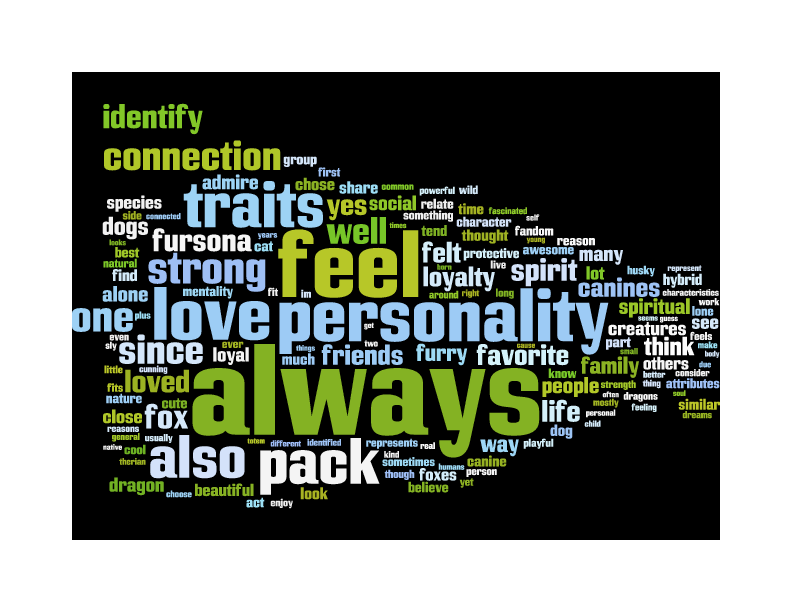
\includegraphics[width=\textwidth]{content/assets/species--wolf}
  \end{center}
  \caption{Wolf word-cloud}
\end{figure}

Here we see a shift in the tagged words to `connection', `identify', as well as `personality', which I think shows a different attitude used to approach the problem of species selection when creating a character. Indeed, we see that `spirituality' figures more strongly, along with `pack', `strong', `spirit', and `one'/'alone', while `loyal' and `social' are deemphasized.

Another interesting thing to note is that, among the several species we pulled from the database, some are more strongly marked, such as the previous two, and some are not. Those who chose dragon as their species, do so for many, many different reasons than wolves or huskies.

\begin{figure}
  \begin{center}
    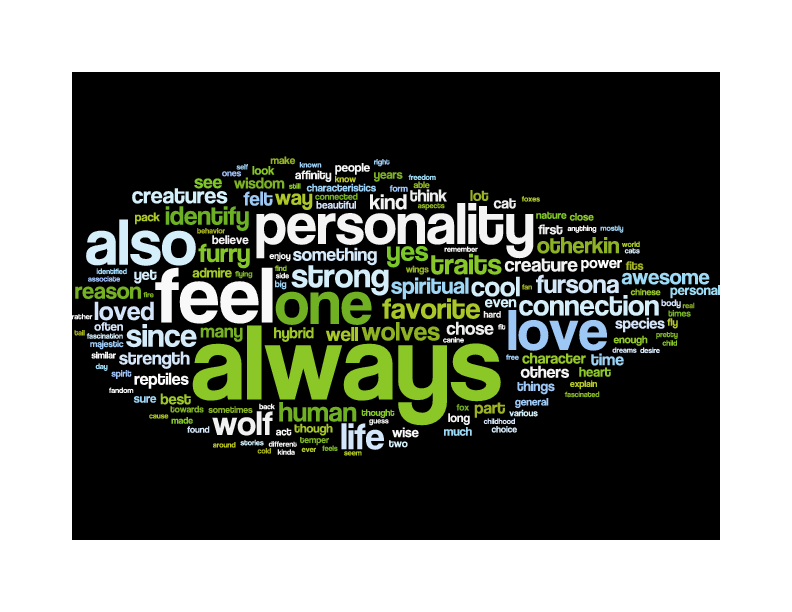
\includegraphics[width=\textwidth]{content/assets/species--dragon}
  \end{center}
  \caption{Dragon word-cloud}
\end{figure}

As you can see, there is less polarization around certain terms, both emotionally marked and the previously tagged words; that is, the cloud is more homogeneous. There are a few potential reasons for this. One is the possibility that dragons have cultural ties to more than just western culture. Wolves have both a strong mythology surrounding them in the west, as well as the advantage of being important in current events, given the re-homing and conservation efforts surrounding the species in North America.

While dragons do have a mythology attached to them in the west, it's very different than their Eastern interpretations, which will lead to less strongly-marked words and phrases showing up in analysis due to a wider spread. Additionally, while dragons are certainly prominent now in fiction words, they are not nearly as prevalent in current events outside of that setting.

These are just some examples, but I think it goes to show that there are indeed some trends, both general and specific, that go into species selection among furries. That's only part of what goes into the creation of a personal character, though, as I think we might achieve some similar results by asking ordinary people to justify their choice of their favorite animal. Thus, during the panel, we also discussed the processes of character creation, growth, and change.

One exercise that I think works well is imposing artificial restrictions. This was, after all, one of the foundations for the literary group Oulipo, of A Void fame (A Void being a book written originally in French entirely without the letter `e', and then, perhaps even more impressively, translated into English with the same restriction in place). By imposing on ourselves restrictions, we reduce the problem of unfettered, and thus directionless, creativity. In that vein, I asked participants to describe their personal characters -- fursonae, if you will -- in one sentence or less. The results are telling:

\begin{quote}
  My persona is a reflection of myself ahead in life which I can use as a goal.
\end{quote}

and

\begin{quote}
  My fursona is an extension of myself as I move forward in life.
\end{quote}

Some were more verbose and specific along these lines:

\begin{quote}
  It's a coping mechanism, a way to become someone else and not deal with tough times, or even provide an outside perspective on them.
\end{quote}

and

\begin{quote}
  Who I strive to become, always a step ahead of me; as I gain attributes, my character stays one step ahead of me. It is my role-model.
\end{quote}

Some people got even more creative:

\begin{quote}
  The person with whom I speak.
\end{quote}

or

\begin{quote}
  Convenient, exaggerated wish fulfillment.
\end{quote}

or simply,

\begin{quote}
  Me.
\end{quote}

The theme of ``a better version of me'' was repeated quite often when discussing both the ways in which characters are created, and the ways in which they change. I really think that this reflects well on us as a subculture. A lot of my focus, when interacting with other furries, is centered around being what I see as an ideal version of myself, as well as just a fox-person. Some of that's simple and mechanical: ``I wish I were able to more clearly express my ideas'' and ``I wish I were more glib, quippier'' are both aided by social interaction through a text-based interface such as one might find online. Beyond that, however, by being able to have this version of myself that is better than me, I, as others mentioned, have something to strive for, something to grow into.

Discussion along these lines continued after the panel itself, as a few of the attendees convinced me to head out to dinner rather than straight up to bed (thanks for that, it was the first real meal of the day). While we ate, we talked about what people took away most from the panel, and also came up with a few additional ideas to help tie together the two ideas of species and character.

One thing that came up was the idea that some gentle joking about species, a sort of lampshading of stereotypes, helps to reinforce species identity with regards to character. Much, if not most of this, as pointed out by Klisoura later on, is self-deprecatory. This helps to forge familiarity between people, especially among members of the same subculture, or even sub-groups within that subculture. Making fun of the chase-instinct in dogs by, as my roommate (a husky) puts it, ``huffing the scent of a new can of tennis balls'', or the face-first pouncing of foxes lending to the overall silliness of the species helps not only to strengthen one's identity with that species but also to provide a conversational starter among friends, or friends-to-be. This can, of course, be mis-applied or simply go too far. The idea that wolves are a dime-a-dozen, or that foxes are all ``sluts'' are complex and sometimes self-reinforcing stereotypes that, by virtue of their being stereotypes, can rub many the wrong way and cause no small amount of offense.

We also noted another interesting conclusion from the panel. Every time I run the ``Exploring the Fandom Through Data'' panel, I bring up the idea of doxa -- that which we accept as truth without requiring proof -- and how sometimes it needs to be challenged when that which is accepted is not necessarily true. For me and several others, one aspect of doxa in particular was challenged during the convention, and it was particularly surprising that this was the case.

One of the attendees at the panel brought up the fact that, during a time of crisis, epiphany, or great change in life, sometimes one's character also goes through change (in this case, a change in species from fox to rat), in a sense reflecting external events in an extreme way. Even though several of us were surprised that such things as a turning point in life would be shown in something so fundamental as one's species, it's one of those things that makes sense upon consideration. Even looking back, for myself, the one time I truly changed species surrounded a profound change in my life. Moving to college -- and all that is entailed in that, such as moving away from parents, getting a job, and so on -- affected me deeply. That signified a total restructuring of my life, even to the point where the old character I had inhabited, a red fox with two tails, the tips of which were dyed green, no longer applied. It was high-school-me. It was me-growing-up. It is not me now.

The reactions from around the room echoed my sentiment. While most were surprised and intrigued at the concept of an external factor such as a move or an epiphany having so large an effect on someone as to cause a sudden, major restructuring of their furry identity, many, myself included, confirmed that this is not infrequent. Those who were most surprised felt that a sudden crisis such as this would not lead to a major change, but rather influence the direction in which their character grew. That is, their goals would change both for them as well as their character, though aspects such as species would remain. Unfortunately, we ran low on time before we had the chance to investigate the differences in how these two rough groups dealt with their character's identity, though it is worth investigating! That there is even the trope of the species-change-journal on FA is proof of this.

As a meta-furry resource, [adjective][species] explores a lot of topics surrounding furry, though it seems of late that the focus has been on topics that happen to be ancillary to the fandom itself. These are all dreadfully interesting, I think, but so is much of the stuff at the core of our subculture, this base layer that helps make us who we are. These are the reasons we seek to meet up together at cons such as RMFC, not simply these supplementary reasons such as being ahead of or behind the rest of the world, any skews in sexual orientation or gender, or even movies about cheetahs, though they may all help. These core facets are worth exploring, as they help to form coherence among all these different animal-folk.

If you are interested in more from the panel, the notes are available here.(ref)
